\chapter{Introduction}%
\label{chap:introduction}
\textit{
This chapter narrows the broad field of robotics down to a largely unsolved problem. After an introduction of that problem, it is defined, associated challenges are listed and state of the art methods are discussed.\bs
}

For robots it remains a hard problem to navigate and act in new, unseen environments. Most approaches controlling the robot and acting as the robot brain fall in one of two categories. The bulk falls into hierarchical approaches~\cite{kaelbling_hierarchical_2011,scholz_navigation_2016,krontiris_dealing_2015}, an hierarchical structure generally consists of an high-level and low-level component. The high-level task planner tries to understand and model the environment, such gained knowledge is used to generate action sequences toward a desired goal. The high-level planner sends actions to a low-level module, that takes care of sending input signals toward the robot actuators. The high-level planner has a prediction horizon consisting of an action sequence, a long prediction horizon compared to the low-level planner which prediction horizon is maximal one single action. Hierarchical structures genarally provide solutions which are computationally effecient but are hierarchical solutions, meaning the solutions found are are teh best feasible solutions in the task hierarchy they search. The quality of the solution depends on the hierarchy which are typically hand-coded and domain specific~\cite{vega-brown_asymptotically_2020}. Altanively to hierarchical approaches, solutions can be provided by searching in a joint configuration space of the robot and objects, where the robots configuration space is augmented with environment objects configuration spaces whilst also including dynamic constraints~\cite{hauser_multimodal_2010,berenson_manipulation_2009,jaillet_path_2013}. Such a joint configuration space suffers from a combinational explosion and it is practically impossible to find a path connecting a start to target configuration. Becuase an action sequence from searching in a joint configuration is exaustive, simplifications are leveraged, for example a search close to the the current configuration, let the robot track this incomplete solution toward a desired goal and search the joint configuration space again close to the new current configuration. Different techniques exist to prevent searching in the entire joint configuration space.\bs

Robots in new unforeseen environments is a broad topic, let's narrow down the scope. The focus lies on the challenging and largely unsolved problem of navigation among movable objects in unknown environments. Consider a simple robot without grippers or arms attached in an environements with movable objects. By sending input toward the wheels the robot can drive around. The environment consists of a flat ground plane, the robot and movable objects. By driving against objects the robot can manipulate objects.\bs 

This creates two different modes of dynamics (driving, pushing) where different differential constraints apply to the different modes. Because there is a discontinuity in the constraints the joint configuration space is a piecewise-analytic configuration space, which hardens motion planning considerably~\cite{vega-brown_asymptotically_2020}. Whilst the robot can interact with the objects in the environment, there is no prior information provided to the robot (e.g. weight, friction coefficient) other than the shape and pose of the object. By interaction with objects the robot can generate a system model, describing the expected trajactory of an object as result of a push from the robot. The robot is tasked to relocate a subset of objects by means of pushing objects. \bs

Applicable to such an robot environment three topics in robotics investigated, these topics are \textbf{\ac{NAMO}}, \textbf{nonprehensile manipulation planning}, and \textbf{learning object dynamics}. Individually a considerable amount of research is done in these topics (\ac{NAMO}~\cite{wang_affordancebased_2020,lavalle_planning_2006,elbanhawi_samplingbased_2014,kingston_samplingbased_2018,chen_fast_2018,ellis_navigation_2022}, nonprehensile manipulation planning~\cite{arruda_uncertainty_2017,mericli_pushmanipulation_2015,toussaint_sequenceofconstraints_2022,stuber_let_2020,stuber_featurebased_2018,bauza_dataefficient_2018}, learning object dynamics~\cite{seegmiller_vehicle_2013,cong_selfadapting_2020}), combining one topic with another is lesser researched and combining all three topics even scarcer.\bs

Combining learning, driving and pushing can improve the driving and pushing skills of the robot. Learning is crucial for unforeseen environments, for example during space exploration. Non-prehensile pushing compared to prehensile pushing saves weight, and for robot with a gripper the ability for nonprehensile pushing comes in handy when the gripper is already in use, for example when a robot relocates a package with it's gripper, it encounters a blocked path by unknown object. Blocked paths and changing environments often coincide, such as a fallen package in a warehouse spilled fluid on the floor, with learning the robot can account for the slippery floor. Finally learning may improve single actions, but it may also improve long term action planning.\bs

\citeauthor{vega-brown_asymptotically_2020} investigated \ac{NAMO} in a piecewise-analytic configuration space to relocate objects~\cite{vega-brown_asymptotically_2020}. Whilst an an optimal plan is obtained with probability one with infinite samples, the algorithm does not learn the pushing relation between the robot and the objects. The ability to learn push dynamics greatly broadens the variety of objects a robot can push. Realisticly robots in warehouses, hospitals or supermarkets might encounter a variety of different objects, but learning dynamics inavitably leads to system model mismatch. An motion planning algorithm should be competable with learned system models and take model mismatch into account. Learning dynamics is a topic untouched by \citeauthor{vega-brown_asymptotically_2020}, because the robot can rigidly grasp the box, so that the robot-box pair behave as a single rigid body as long as the box is grasped. This model avoids the complexity of real world pushes, becoming alienated with reality.\bs

\citeauthor{wang_affordancebased_2020} takes nonprehensile manipulation planning out of the equation and only focussus on the \ac{NAMO} problem and learning system dynamics. Learning interaction by embedding unknown objects with affordance information followed by planning with a contact-implicit motion planner toward a robot goal location~\cite{wang_affordancebased_2020}. By removing push manipulation, finding a path from a start to target configuration simplifies, only a single mode of dynamcis is contained in the configuration space and the piecewise-analytic configuration spaces becomes a configuration space. There exist a variety of sampling-based motion planners that can find a path with properties such as probabilistic completeness, replanning in dynamic environments, planning under uncertainty or asymtotically optimality~\cite{karaman_samplingbased_2011,elbanhawi_samplingbased_2014}. Challenging problems introduced by push manipulation are removed by simply removing push manipulation.\bs

\citeauthor{vega-brown_asymptotically_2020} combined \ac{NAMO} with nonprehensile manipulation panning, \citeauthor{wang_affordancebased_2020} combines \ac{NAMO} with learning system models. Both combine 2 of the 3 topics allowing for an more in depth analysis but avoiding the problems introduced by combining all 3 topics (\ac{NAMO}, nonprehensile manipulation plannning and learning system models). \citeauthor{sabbaghnovin_model_2021} does combine all three topics. She proposes to obtain system models by analysing and converting a limited set of robot-object test pushes using Bayesian regression to predict model parameters. Path planning is the result of solving an proposed mixed-integer convex optimization~\cite{sabbaghnovin_optimal_2016} which is tracked by \ac{MPC} control, the proposed method is tested in a hospital setting~\cite{novin_dynamic_2018} and was later improved upon resulting in lowering trajectory errors~\cite{sabbaghnovin_model_2021}.\bs

Since \citeauthor{sabbaghnovin_model_2021} uses a gripper to manipulate objects, the reseach falls into the category prehensile manipulation. Prehensile manipulation in comparinson with nonprehensile manipulation is simpler because a pushed object becomes disconnected easier compared to a gripped object. Her research is specific to legged objects, which limits the set of objects to manipulate considerably.\bs

This thesis proposes a method where the robot should learn robot and object dynamics by interaction, perform motion and manipulation planning whilst facing a wide variety of objects, tasks and environments. The 3 topics (\ac{NAMO}, nonprehensile manipulation plannning and learning system models) are bundled together with a technique known as \textbf{backward induction} also known as \textbf{backward tracing} or \textbf{backward search} (this thesis will refer to this technique with the term backward search). The proposed method in this thesis and \citeauthor{sabbaghnovin_model_2021} proposed method solve comparible problems using different techniques, allowing for easy comparinson between the the results of \citeauthor{sabbaghnovin_model_2021} and the results from the proposed method in this thesis.\bs

\section{Research Question}%
\label{sec:research_question}
In order to investigating the effect of learning on action selection and on action planning the following reseach questions have been selected.\bs

\textbf{Main research question:}
\begin{center}%
\label{researchquestion:main}
\large
How do learned objects' system models improve global task planning\\for a robot with nonprehensible manipulation abilities over time?
\end{center} 

The main research question is split in two smaller more detailed subquestions. Essentially the first research subquestions asks: \quotes{how does the proposed method work?}, that allows to explain the proposed method. The second research subquestion essentially asks: \quotes{How does it compare to similar existing methods?}, allowing to compare the proposed methods with existing state-of-the-art methods by comparing their results.\bs

\textbf{Research subquestion:}
\begin{enumerate}
    \item\label{researchsubquestion:does_it_work} Can the proposed method combine learning and planning for push en drive applications with a technique known as backward search~\cite{krontiris_dealing_2015}?
    \item\label{researchsubquestion:does_it_compare} How does learning system models and remembering interactions compare to only learning system models? And, how does the proposed method compare against the state of the art? 
\end{enumerate}

Answering the research subquestions provides a solid base to answer the main research question. The main research question is aimed to test robot abilities in a new environment, and track improvement in that a new environment. Some questions which come up are: Will the robot prefer specific strategies for certain objects?, How much improvement will a robot make with some experience?. Will the robot converge to a preferred strategy for an object, and will it converge the same strategy again if it's memory is wiped.\bs

\section{Problem Description}%
\label{sec:problem_description}
To answer the research questions, test will be performed in a robot environment. A simple environment is desired because that will simplify testing, yet the robot environment should represent many real world environment in which robots operate. For the environment a flat ground plane is selected, since many mobile robots operate in a workspace with a flat floor, such as the supermarked, warehouses or distrubution centra's. The robots to tests should be flat robots, that lowers the chance of tipping over. A 3 dimensional environment is selected, but with a flat floor and a flat robot can be threated as a 2 dimensional problem, because the robot and objects can only change position over $x$ and $y$ axis ($xy$ plane parallel to the ground plane) and rotate around the $z$ axis (perpendicular to the ground plane).\bs

Let's start with defining the environment.\\Let the tuple $\left\langle \text{Origin}, \text{Ground Plane}, \text{Ob}, E \right\rangle$ fully define a robot environment where:\bs

\par\smallskip\noindent
\centerline{\begin{minipage}{0.8\textwidth}
\begin{enumerate}
  \item[Origin] Static point in the environment with a $x$-, $y$- and $z$-axis. Any point in the environment has a linear and an angular position and velocity with respect to the origin \vspace{0.5\baselineskip}
 \item[Ground Plane] A flat plane parallel with the Origin's $x$- and $y$- axis. Objects cannot pass through the ground plane and meet sliding friction when sliding over the ground plane. \vspace{0.5\baselineskip}
 \item[Ob] A set of objects, $\text{Ob} = (obst_1, obst_2, obst_3, \dots, obst_i)$ with $i>1$, an object is an 3-dimensional body with shape and uniformly destributed mass. Examples of objects are given in \cref{fig:example_objects}. \vspace{0.5\baselineskip}
  \item[$E$] A set of motion equation describing the behaviour of objects such as gravity, interacteraction with the ground plane or interaction with other objects. The motion equations are equivalent to the true dynamics. \vspace{0.5\baselineskip}
\end{enumerate}
\end{minipage}}
\par\smallskip

A state consists of the linear and angular position and velocity of a point with respect to the environment's origin.\bs

Formally, a \textbf{state}, $s_{id}(k)$ is a tuple of $\left\langle pos_x(k), pos_y(k), pos_\theta(k), vel_x(k), vel_y(k), vel_\theta(k)\right\rangle$\\ where $pos_x, pos_y, vel_x, vel_y, vel_\theta \in \mathbb{R}, \quad  pos_\theta \in [0, 2\pi)$, \quad $k$ indicates the time step and can be removed for simplicity if the state remain constant for all $k$.\\

\subsection{Task}%
\label{subsec:task}
The research questions want to investigate the effect of learning system models, and monitor the effect of learned knowledge over time. Thus the robot needs an incentive to learn object properties, and interactions with the objects in it's environment, otherwise it would simply remain standing still on it's initial location. Therefore the robot is asked to complete a task. A task is defined as a subset of all objects with associated target states:\bs
\[\text{task} = \left\langle Obst_{task}, S_{targets} \right\rangle\]

where $Obst_{task} = (obst_1, obst_2, obst_3, \dots, obst_k) \subset Ob$, $S_{target} = (s_1, s_2, s_3, \dots s_k)$ and $k>0$\bs

A task is completed when the robot manages to push every object to it's target position within a specified error margin. 

\subsection{Assumptions}%
\label{subsec:assumptions}
A complex robot environmnet is not required to answer the research questions. Therefore influences other than the robots are neglected, some real world dynamics which are generally negligable are neglected, a workaround is found to measure uncertain properties and the objects in the environment will not tip over. To simplify the pushing and learning problem, a number of assumptions are taken, which are now listed.\bs

\begin{assumption*}%
\label{assumption:closed_world}
\textbf{Closed-World Assumption:} Objects are manipulated, directly or indirectly only by the robot. Objects cannot be manipulated by influences from outside the environment.
\end{assumption*}\bs

\begin{assumption*}%
\label{assumption:quasi_static}
\textbf{Quasi-Static Assumption:} Velocities are small enough that inertial forces are negligible~\cite{stuber_let_2020}.
\end{assumption*}\bs

\begin{assumption*}%
\label{assumption:perfect_object_sensor}
\textbf{Perfect Object Sensor Assumption:} the robot has full access to the poses and geometry of all objects in the environment at all times.
\end{assumption*}\bs

\begin{assumption*}%
\label{assumption:order_does_not_matter}
\textbf{Tasks are Commutative Assumption:} Tasks exist of multiple objects with specified target positions. The order in which objects are pushed toward their target position is commutative.
\end{assumption*}\bs

\begin{assumption*}%
\label{assumption:no_tipping}
\textbf{Objects do not tip over Assumption:} Movable objects slide if pushed.
\end{assumption*}\bs

The assumptions taken serve to simplify the problem of task completion. Note that in \cref{sec:future_work} insight is given to remove all assumption except the quasi-static assumption. By removing assumptions completing tasks becomes a harder problem, but a more realistic problem closer to the real world applications.\bs

Assumptions might have certain implications, which are now listed. The \hyperref[assumption:closed_world]{\textbf{closed-world assumption}} implies that objects untouched by the robot and with zero velocity component remain at the same position. Completed subtasks are therefore assumed to be completed for all times after completion time.\bs

The \hyperref[assumption:quasi_static]{\textbf{quasi-static assumption}} allows to neglect complex dynamics, which in many cases are negligible. To ensure that complex dynamics do not become significant during testing, a maximum robot speed or accelaration is enforced.\bs

The \hyperref[assumption:perfect_object_sensor]{\textbf{perfect object sensor assumption}} simplifies a sensor setup, it prevents Lidar-, camera setups and for tracking setups with aruco or other motion caputer markers. The existence of a single perferct measurement wipes away the need to combine measurements from multiple sources with sensor fusion algorithms, such as Kalman filtering \cite{verhaegen_filtering_2007}.\bs

Certain tasks are only feasible if performed in a certain order (e.g. the Tower of Hanoi), the \hyperref[assumption:order_does_not_matter]{\textbf{tasks are commutative assumption}} allows to focus only on a single subtask since it does not affect the completion or feasibility of other subtasks.\bs

The \hyperref[assumption:no_tipping]{\textbf{objects do not tip over assumption}} ensures that objects do not tip over and suddenly have vastly different dynamics. In practice objects will not be higher than the minimum width of the object, and spheres are excluded since rolling essentially is tipping. 

\paragraph{Robot and Objects, an Example}
To get a sense of what the robots and the objects look like, see the two robot's that are used during testing in \cref{fig:example_robots}. And among many differnt objects two example objects displayed in \cref{fig:example_objects}.

\begin{figure}[H]
    \centering
    \begin{subfigure}{.5\textwidth}
    \centering
    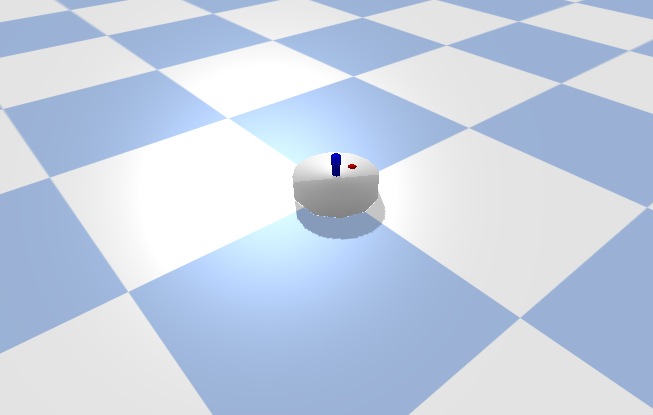
\includegraphics[width=0.8\textwidth]{figures/point_robot.png}
    \caption{The holonomic point robot\\the 2 velocity inputs drive the robot in $x$ and in $y$ direction}%
    \label{subfig:example_point_robot}
    \end{subfigure}%
    \begin{subfigure}{.5\textwidth}
    \centering
    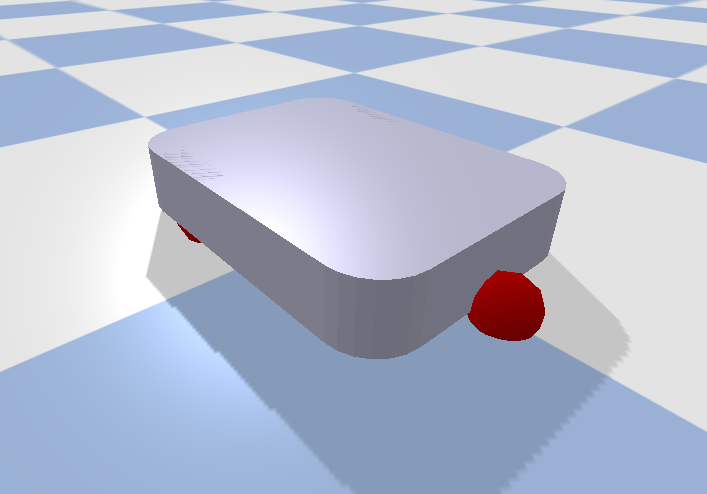
\includegraphics[width=0.8\textwidth]{figures/boxer_robot.png}
    \caption{The nonholonomic boxer robot\\the first velocity input drives the robot forward/backward\\the second rotates the robot}%
    \label{subfig:example_boxer_robot}
    \end{subfigure}%
    \caption{Robots used for testing the proposed method}%
    \label{fig:example_robots}
\end{figure}

\begin{figure}[H]
    \centering
    \begin{subfigure}{.5\textwidth}
    \centering
    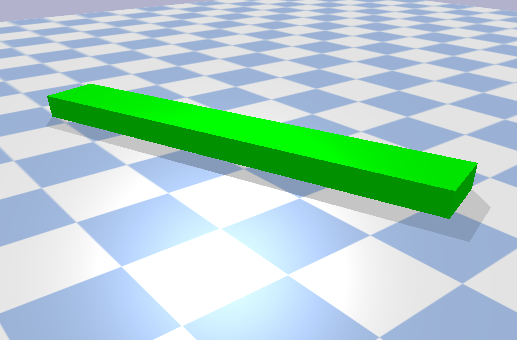
\includegraphics[width=0.8\textwidth]{figures/box_object.png}
    \caption{A box object}
    \end{subfigure}%
    \begin{subfigure}{.5\textwidth}
    \centering
    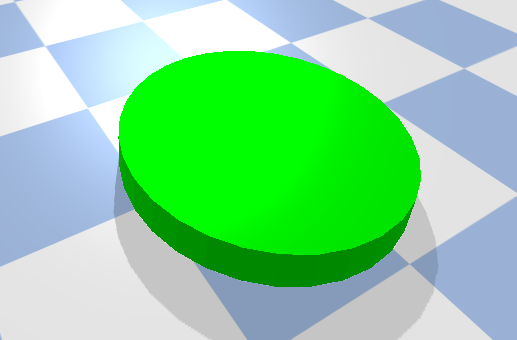
\includegraphics[width=0.8\textwidth]{figures/cylinder_object.png}
    \caption{A cylinder object}
    \end{subfigure}%
    \caption{Various objects in the robot environment}%
    \label{fig:example_objects}
\end{figure}

For complete environments with accompanying tasks, see~\cref{chap:results}.\bs

\subsection{Challenges}%
\label{subsection:problems_with_task_planning}
Finding a solution to a task as is defined in \cref{subsec:task}, inside an robot environment defined in \cref{sec:problem_description} bears some challenges. In this section the main challenge is highlighted and other subchallenges are introduced. Finding a solution requires overcoming the main and subchallenges. Before listing the challenges that this thesis will take on, a challenge is presented that seves to show the difficulty of finding an optimal solution to a task.\bs

Assuming the task has at least a one object to place at a target state (exclude purely \ac{NAMO} problems), finding an optimal solution to a task is \ac{NP-hard} since, it can be reduced to the piano mover's problem which is known to be \ac{NP-hard}~\cite{reif_motion_1985}.\\Problems in class P have an solution which can be found in polynomial time, problems in \ac{NP} are problems for which a solution cannot found in polynomial time. For problems in \ac{NP}, when provided with a solution, verifying that the solution is indeed an valid solution can be done in polynomial time. \ac{NP-hard} problems are a class of problems which are at least as hard as the hardest problems in \ac{NP}. Problems that are \ac{NP-hard} do not have to be elements of NP. They may not even be decidable~\cite{pokharel_computational_2020}. This thesis, or other recent studies in the references do not attempt to find an optimal solution. Instead they provide a solution whilst guaranteeing properties such as near-optimality or probabilistic completeness.\bs

Finding a solution to a task requires a search in the \textit{joint configuration space} which comes with 2 problems to tackle. Before investigating a problem, let's investigate how to construct a joint configuration space which is created by augmenting the robot's configuration space with the configuration space of every object. For example, if the configuration space for both robot and objects consist of position $x$, $y$ and orientation $\theta$ around the $z$ axis around the $z$ axis, then the joint configuration space is $3n$-dimensional, where $n$ is the number of objects including the robot. The joint configuration space's dimensionality grows linearly, meaning the joint configuration space grows exponentially in the number of objects, which is an explosion in the number of possible combinations the environment can be in, the enormity of teh joint configuration space is the root of the main challenge.\bs

Unspecified target positions are a fine example of the curse of dimensionality, consider a blocked corridor. The object needs to be pushed to free the path but the target location of this object is unspecified, as long as the robot can drive through the corridor unhindered. A solution is, the robot drives to the object, pushes the object, and then drives through the corridor. The push action influences the free space where the robot has to drive in when the push action was completed. Even sampling-based search algorithms cannot computationally find a path between a start en target state in joint configuration space in reasonable time (orders of magnitude slower than real-time). Only by leveraging simplifications of the joint configuration space a search be performed, such as discretization~\cite{sabbaghnovin_optimal_2016}, factorization~\cite{vega-brown_asymptotically_2020} or a heuristic function combined with a time horizon~\cite{sabbaghnovin_optimal_2016}. Such techniques prevent searching in configurations relatively far from the current configuration, while optimality guarantees can be given and real-time implementations have been shown.\bs

The second problem is that the joint configuration space is \textit{piecewise-analytic}. Let's eleborate, when the robot drives constraints apply due to e.g.~the robot being nonholonomic. When the robot pushes an object a different set of constraints are applicable, creating 2 different modes of dynamics. A configuration space containing multiple modes of dynamics is an piecewise-analytic configuration space~\cite{vega-brown_asymptotically_2020}. Motion planners have great difficulty with crossing the boundary from one mode of dynamics to another.\bs

The main challenge is to find, for a given task, a path from a starting configuration of the environment (the point in the joint configuration space that the environment starts in) to a desired target configuration in joint configuration space, where all specified objects are at their target state as specified in the task. Whilst finding such a path requires searching a enormous joint configuration space that is piecewise analytic. The proposed solution will essentially avoid searching directly in the joint configuration space and will search in subspaces of the joint configuration space were only a single mode of dynamics is present. Subchallenges that emerge are system identification, control methods, estimating path existence, motion and manipulation planning, these subchallenges will be properly introduced and eleborated on in \cref{chap:hgraph_and_kgraph}.\bs

\section{Report Structure}%
\label{sec:report_structure}
\todo[inline]{Create the report structure when the report structure does not change any more}


